\chapter{初段ミューオントリガーシステム}








\begin{figure}[tb]
  \centering
  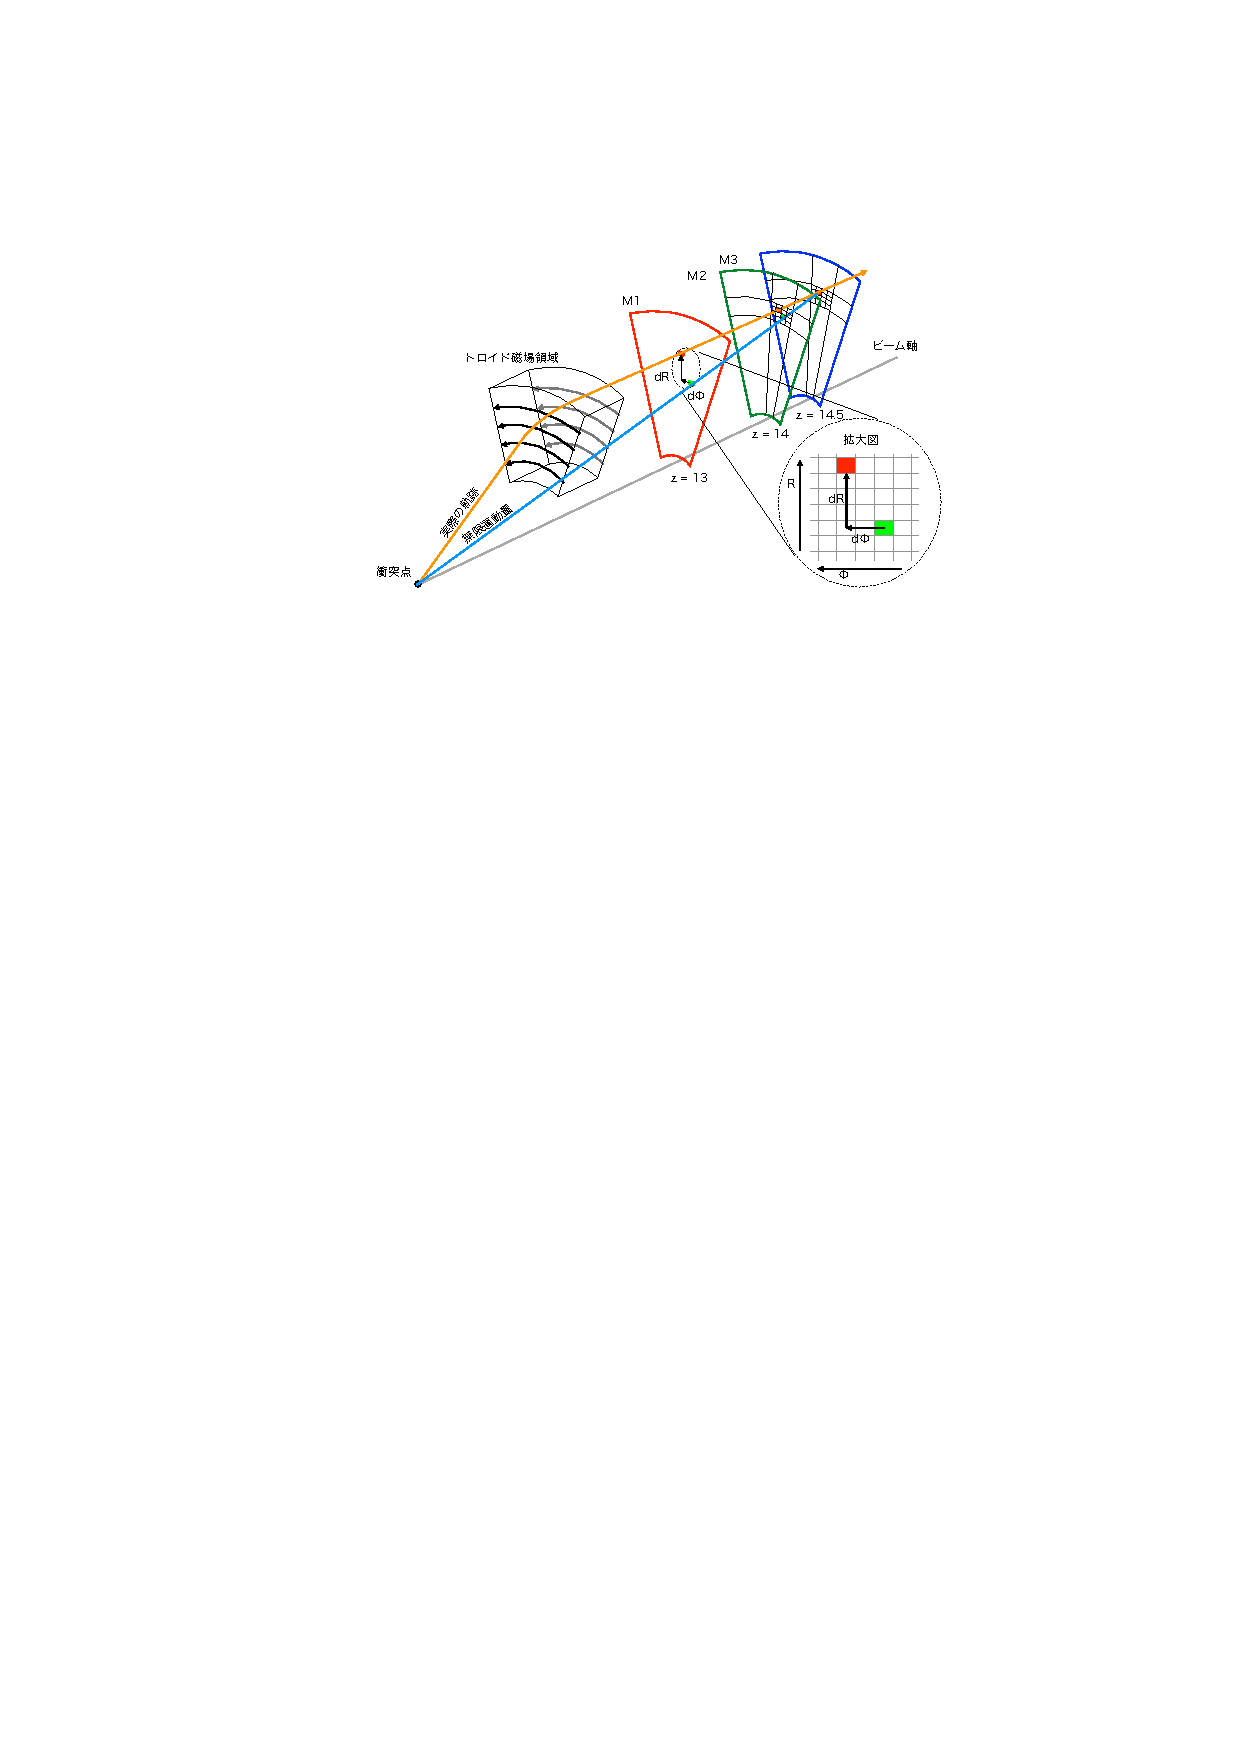
\includegraphics[clip, width=14cm]{fig/3/akatsuka_mt_trigger_scheme.pdf}
  \caption{ATLAS検出器エンドキャップ領域におけるトリガースキームの概念図\cite{article:akatsuka-mron}。無限大の運動量を持つミューオンを仮定し、磁場によって曲げられたミューオンとの位置の差を用いて$\pt$を計算する。}
  \label{fig:trigger-scheme}
\end{figure}









